\section{Vesting Schedule}

\label{sec:vesting}
% ============================================================================

\begin{table}[H]
\centering
\small
\begin{tabular}{lrrrr}
\toprule
\textbf{Category} & \textbf{Cliff} & \textbf{Vest} & \textbf{TGE} & \textbf{Total} \\
\midrule
Community & --- & 20 yr & 5\% & 400M \\
Team & 12 mo & 48 mo & 0\% & 200M \\
Treasury & --- & DAO & 10\% & 150M \\
Infrastructure & 6 mo & 36 mo & 5\% & 150M \\
Liquidity & --- & --- & 100\% & 100M \\
\bottomrule
\end{tabular}
\caption{Vesting summary. TGE = tokens unlocked at Token Generation Event. Community tokens emit via mining schedule over 20 years.}
\label{tab:vesting}
\end{table}

At TGE, the circulating supply is:
\begin{equation}
S_{\text{circ}}(0) = 0.05 \times 400\text{M} + 0 + 0.10 \times 150\text{M} +
0.05 \times 150\text{M} + 100\text{M} = 142.5\text{M},
\end{equation}
representing 14.25\% of total supply. This controlled initial float limits sell
pressure while providing sufficient liquidity for trading and compute payment.

\subsection{Unlock Schedule}

The cumulative unlock follows a piecewise-linear trajectory:

\begin{center}
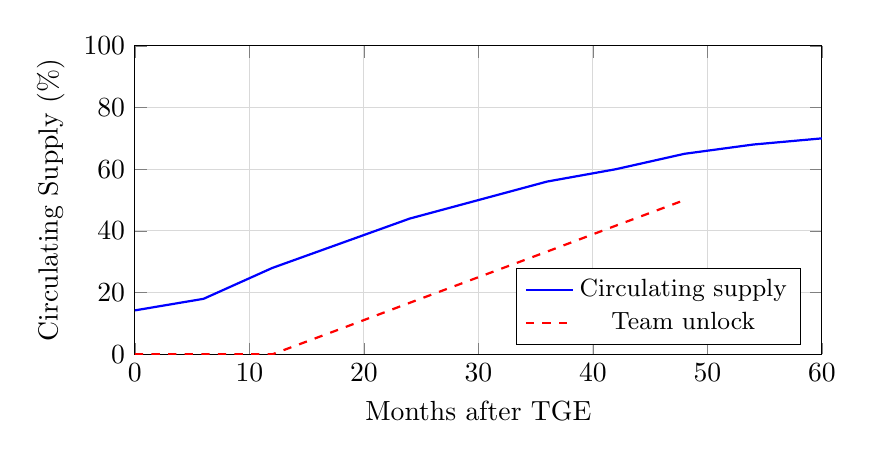
\begin{tikzpicture}
\begin{axis}[
    width=0.85\linewidth,
    height=5.5cm,
    xlabel={Months after TGE},
    ylabel={Circulating Supply (\%)},
    xmin=0, xmax=60,
    ymin=0, ymax=100,
    grid=major,
    grid style={gray!30},
    legend pos=south east,
    legend style={font=\small},
]
\addplot[thick, blue, mark=none] coordinates {
    (0, 14.25)
    (6, 18)
    (12, 28)
    (18, 36)
    (24, 44)
    (30, 50)
    (36, 56)
    (42, 60)
    (48, 65)
    (54, 68)
    (60, 70)
};
\addlegendentry{Circulating supply}
\addplot[thick, red, dashed, mark=none] coordinates {
    (0, 0)
    (12, 0)
    (18, 8.3)
    (24, 16.7)
    (30, 25)
    (36, 33.3)
    (42, 41.7)
    (48, 50)
};
\addlegendentry{Team unlock}
\end{axis}
\end{tikzpicture}
\end{center}

% ============================================================================
